\documentclass{book}
\usepackage{xeCJK}
\usepackage{ctexcap}
\usepackage{bm}
\usepackage{amsmath,amssymb,amsfonts}
\usepackage{float}

\begin{document}
\chapter{变压器的类别和结构}
\section{变压器的主要类别}
变压器是一种静止的电机,它的主要作用是通过电磁感应把一种电压等级的交流电能转变为同频率的另一种电压等级的交流电能。在电力系统中,变压器对电能的经济传输、灵活分配和安全使用具有重要意义。此外,在电量测量、控制和某些特殊用电设备上也大量应用着各种类型的变压器。

为了适应不同的使用目的和工作条件,不同类型的变压器在结构和性能上有很大的差异。通常可按用途、相数、结构特点和冷却方式进行分类。
\subsection{按用途分类}
(1)电力变压器:用于电力系统中,可分为升压变压器、降压变压器、配电变压器、联络变压器等。
将10kV配电网升压改造成20kV供电方式,将是一个长期渐变的过程。在这个过程中,势必会存在10kV配电网与20kV配电网共存的一个过渡时期,这就要求我们在建设20kV电网的同时,兼顾对已有的10kV配电系统继续供电,进而逐步将10kV配电网络改造为20kV供电。联络变压器可以满足小容量、小范围区域的供电,具有主接线简单可靠、占地面积小、投资少、建设周期短等优点,可以现有的10kV配电网络及新建的20kV配电网得到充分利用。
(2)特殊变压器:如整流变压器、电炉变压器、电焊变压器。

整流变压器是整流设备的电源变压器。整流设备的特点是原边输入交流,而副边输出通过整流元件后输出直流。 作为整流装置电源用的变压器称为整流变压器。工业用的整流直流电源大部分都是由交流电网通过整流变压器与整流设备而得到的

专为各种电炉提供电源的变压器。工业用电炉变压器大致可分为3类:电阻炉变压器、电弧炉变压器和感应炉变压器。

电焊变压器是一种双绕组变压器。为了调节电弧点火电压,原绕组配备分换出头,用一分接开关来调节副边的空载电压。原、副绕组分装在两个铁心柱上,使变压器本身具有较大的漏电抗,因而副边的端电压将随电流的增大而激剧下降。副绕组电路中串联一个铁心电抗器,供调节焊接电流大小之用。改变电抗器空气隙的长度,电流将随着空气隙的增长而增大。

(3)仪用互感器:包括电压互感器和电流互感器。

(4)试验用变压器:主要包括调压变压器以及电压很高、电流很小的高压试验用变压器。
\subsection{按相数分类}
(1)单相变压器:用于改变单相交流电压。

(2)三相变压器:用于改变三相交流电压。

(3)多相变压器:用于特殊场合。
\subsection{按每相绕组数目分类}
(1)双绕组变压器:每相有一个高压绕组和一个低压绕组。

(2)自耦变压器:每相只有一个绕组,低压绕组是高压绕组的一部分。

(3)三绕组变压器:每相有高压、中压、低压三个绕组。

(4)多绕组变压器:每相绕组多于三个。
\subsection{按冷却方式分类}
(1)干式变压器:变压器铁心和绕组直接与空气接触,通过空气的对流将产生的热量散掉。

(2)油浸式变压器:变压器的铁心和绕组全浸在变压器油中,通过变压器油的流动将热量传至邮箱壁,再散到空气中去。

\section{电力变压器的基本结构}
通常的变压器多为油浸式的,其主要结构部件包括铁心、绕组、油箱及其他附件。铁心和绕组是变压器完成能量转换的核心部分,称为变压器的器身。油浸式变压器的器身安放在充满变压器油的油箱内。下面分别对每种部件进行简要介绍。
\subsection{铁心}
铁心是变压器的磁路部分,包括铁心柱和铁轭。铁心柱上套装高、低压绕组,铁轭将铁心柱连接起来,使之形成闭合此路。由于铁心的磁通为一交流磁通。为了减少涡流损耗,变压器铁心通常用厚度为0.35mm、表面涂绝缘漆的硅铜片叠压而成,叠装前,先按铁心的尺寸将硅钢片剪成几种规格的长方形冲片。为了减少铁心的磁阻。在叠装时相邻两层的冲片接缝要错开,图\ref{fig:2.1}所示为三相变压器铁心相邻两层冲片的排列方法。
\begin{figure}  %两个图片并排放
	\begin{minipage}[H]{0.5\linewidth}  
		\centering  
		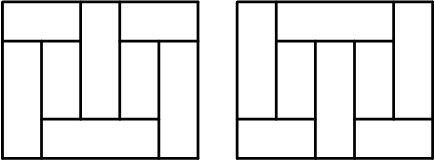
\includegraphics[width=2.2in]{2-1.png}  
		\caption{三相变压器铁心相邻两层冲片排列方法}  
		\label{fig:2.1}  
	\end{minipage}
	\begin{minipage}[H]{0.5\linewidth}  
		\centering  
		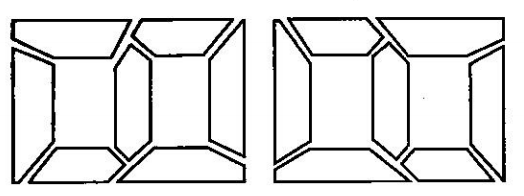
\includegraphics[width=2.2in]{2-2.png}  
		\caption{冷轧硅钢片的斜接缝叠装}  
		\label{fig:2.2}  
	\end{minipage}  
\end{figure}  
冷轧硅钢片的磁性能高于热轧硅钢片,但它有较强的方向性,即只有在磁通沿着轧碾方向流通时才有较高的导磁系数和较小的铁损耗,因此,当铁心采用冷轧硅钢片时,必须采用斜接缝,相邻两层的接缝也错开,如图\ref{fig:2.2}所示,这时如仍按图\ref{fig:2.1}所示下料和叠装,则在磁路拐角处,由于磁通和轧碾方向成90°,将引起磁阻增大、铁损耗增加。

为了使绕组便于制造和在电磁力作用下受力均匀并具有较高的机械强度,一般都把绕组制成圆筒形。而铁心柱的截面则做成图\ref{fig:2.3}所示的阶梯状多边形,以便充分利用绕组内的圆柱形空间。阶梯的级数越多,截面越接近于圆形,空间利用率越高,但制造工艺也越复杂。在实际生产中,变压器的容量越大,所取阶梯的级数越多,而小容量变压器有时还采用正方形截面的铁心柱。

铁轭的截面有矩形、阶梯形等几种,如图\ref{fig:2.4}所示。为了减少变压器的空载电流和铁损耗,铁轭截面一般比铁心柱截面大5\%\textasciitilde10\%。
\begin{figure}  %两个图片并排放
	\begin{minipage}[H]{0.5\linewidth}  
		\centering  
		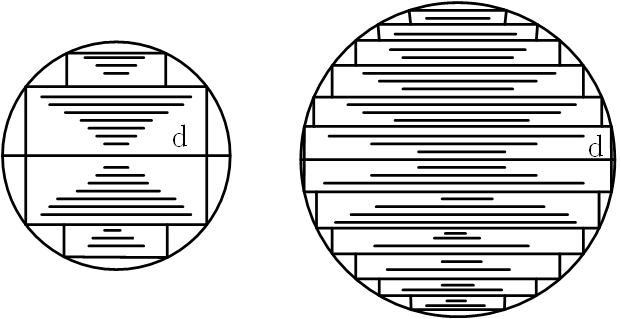
\includegraphics[width=2.2in]{2-3.png}  
		\caption{铁心柱截面的形状}  
		\label{fig:2.3}  
	\end{minipage}
	\begin{minipage}[H]{0.5\linewidth}  
		\centering  
		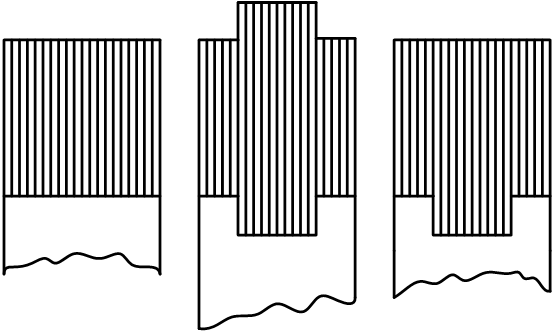
\includegraphics[width=2.2in]{2-4.png}  
		\caption{铁轭截面的各种形状}  
		\label{fig:2.4}  
	\end{minipage} 
\end{figure} 
\subsection{绕组}
绕组是变压器的电路部分,一般用有绝缘包皮的铜线或是铝线绕制而成。变压器工作时接到高压电网的绕组称为高压绕组,接低压电网的绕组称为低压绕组。高、低压绕组之间的相对位置有同心式和交迭式两种不同的排列方式。同心式绕组的低压绕组靠近铁心柱,高压绕组套在低压绕组的外边。交迭式绕组的高、低绕组沿铁心轴线高度方向交替地排列,如图\ref{fig_2.5}所示。在实际变压器中多数为同心式绕组。

根据变压器容量大小和电压等级的不同,同心式绕组可分为圆筒式、连续式、纠结式和螺旋式几种类型。
\begin{figure}[H]
	\centering
	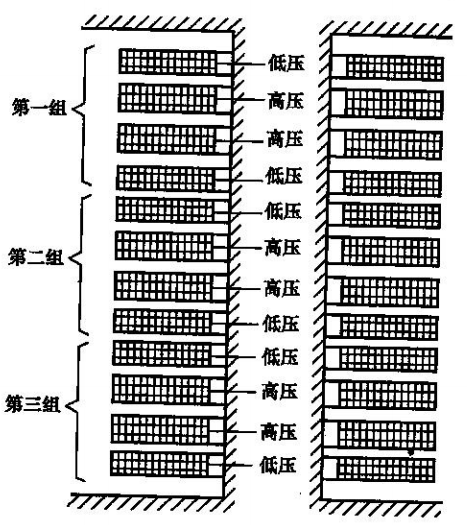
\includegraphics[width=0.80\textwidth]{2-5.png} %0.80表示占texwidth的百分之80
	\caption{散热器内部构造模型}
	\label{fig_2.5}
\end{figure}
\subsection{油箱}
\subsubsection{变压器油}

变压器油的第一个作用是散热,通过油的对流,将绕组和铁心由于损耗而产生的热量传送到油箱壁,再由油箱表面散逸到空气中去。因此,对于一定容量的变压器,必须保证其油箱有足够大的散热表面积。

变压器油的第二个作用是加强绝缘。由于变压器油具有较大的介电强度,当器身全浸在变压器油中时,高、低压绕组之间以及它们与铁心之间的绝缘都将得到加强。变压器油的绝缘性能与它的纯净度关系极大,因此,在使用中必须尽量防止水分和杂质进入变压器的油箱。

\subsubsection{油箱的类型}

(1)平滑油箱。它仅靠油箱本身的表面积散热,用于$50\text{V}\cdot \text{A}$以下的小型变压器。

(2)管式油箱。为了增大散热面积,在油箱周围焊装成排的油管。管式油箱及油箱盖上的各种辅助部件如图\ref{fig_2.6}所示。

(3)散热器式油箱,当变压器容量大于$3000\text{V}\cdot \text{A}$时,在油箱四周已安排不下散热所需的油管。这时先用一定数量的油管组合成一个整体的散热器,然后再将数个这样的散热器安装在油箱的四周。对于容量在$10000\text{V}\cdot \text{A}$以上的变压器,还要在散热器上安装强力通风装置(电风扇)以提高散热能力。图\ref{fig_2.7}所示为具有散热器油箱的变压器外形。

(4)强迫油循环冷却方式。变压器油箱上无油管和散热器,而是通过油泵将变压器热油抽到油箱外边的冷却器中,油冷却后再流回油箱。用于$400000\text{V}\cdot \text{A}$以上的巨型变压器。
\begin{figure}[H]
	\centering
	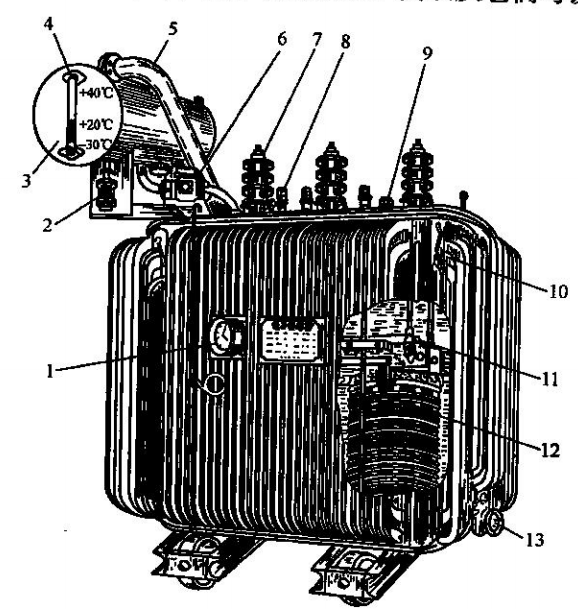
\includegraphics[width=0.80\textwidth]{2-6.png} 
	\caption{管式邮箱及邮箱盖上的各种辅助部件}
	\label{fig_2.6}
\end{figure}1—信号式温度计;2—吸湿器;3—储油柜;4—油表;5—安全气道;6—气体继电器;7—高压套管;8—低压套管;9—分接开关;10—邮箱;11—铁心;12—线圈及绝缘;13—放油阀门
\begin{figure}  %两个图片并排放
	\begin{minipage}[H]{0.5\linewidth}  
		\centering  
		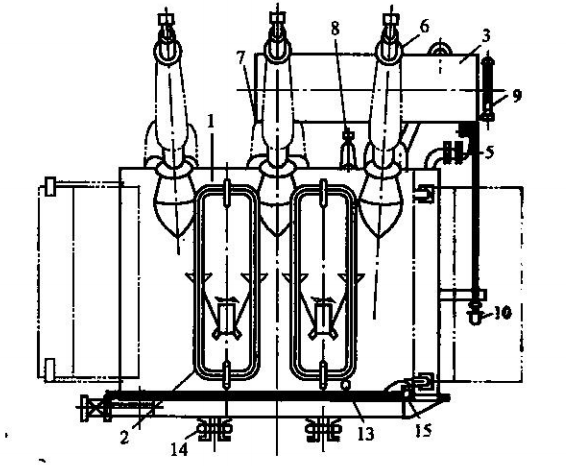
\includegraphics[width=2.2in]{2-7-1.png}  
	\end{minipage}
	\begin{minipage}[H]{0.5\linewidth}  
		\centering  
		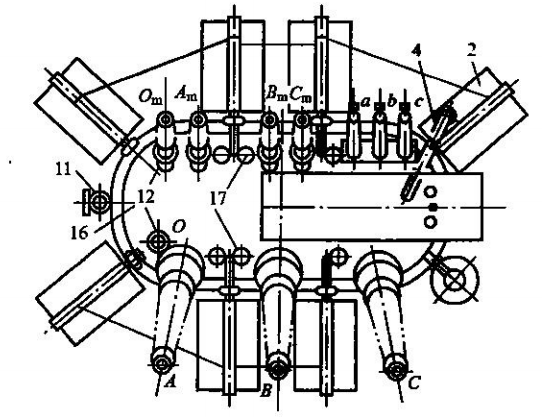
\includegraphics[width=2.2in]{2-7-2.png}  	 
	\end{minipage} 
	\caption{具有散热器邮箱变压器的外形}  
	\label{fig_2.7}
\end{figure} 
1—邮箱;2—散热器;3—油枕;4—排气管;5—气体继电器;6—高压套管;7—中压套管;8—低压套管;9—油标;10—吸湿器;11—事故放油阀门;12—中性点套管;13—接地螺栓;14—滚轮;15—取油样阀门;16—信号温度计;17—分接开关操动机构
\subsection{其他附件}
\subsubsection{储油柜}

为了防止潮气和杂质的侵人,希望油箱内部与外界空气隔离。但如果使油箱本身密闭,则当油受热膨胀时可能造成油箱胀裂。储油柜(俗称油枕)为一圆筒形容器,横放于油箱上 方,用管道与变压器的油箱连通。当变压器油热胀时,油由油箱流向储油柜;当变压器油冷缩时,油由储油柜流向油箱。储油柜油面上部的空气由一通气管道与外部大气相通。通气管 道中放置干燥剂,以减少进人储油柜空气中的水分。储油柜的底部设有沉积器,以沉聚侵入储油柜的水分和污物,定期加以排除。在储油柜的一端还装有油位表以观测油面的高低,当由于渗漏等原因造成油量不足时,应及时注油加以补充。

\subsubsection{气体继电器}

安装在油箱和储油柜的连通管中间,当变压器内部由于故障而产生气体时,它可发出报 警信号或自动切断变压器电源。

\subsubsection{安全气道(也称排气管)}

它是一个长钢管,下端安装在油箱盖上并与油箱内部相连,上端部用一定厚度的玻璃板封死。当变压器内部发生严重故障而产生大量气体时,气体和油流将冲破玻璃板向外喷出,从而防止油箱发生爆裂。

\subsubsection{分接开关}

为了保证二次侧输出电压的变化不超出允许的范围,有时需改变一、二次侧的匝数比。转动分接开关可改变变压器高压绕组的匝数,从而达到调节输出电压的目的。图\ref{fig_2.8}所示为无载调压的原理接线图。中、小型变压器一般有三个分接开关位置。如图\ref{fig_2.8}(a)所示,调节范围为$ \pm 5{\rm{\% }}$;大型变压器一般有五个分接头位置,如图\ref{fig_2.8}(b)所示,调节范围为$ \pm 2.5{\rm{\% }}$和$ \pm 5{\rm{\% }}$。
\begin{figure}[H]
	\centering
	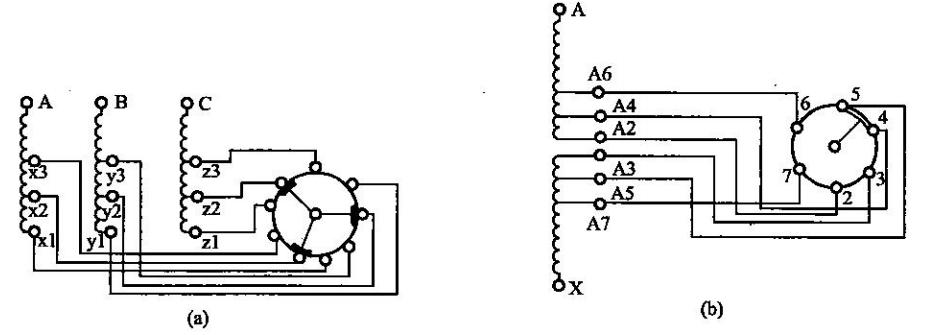
\includegraphics[width=0.80\textwidth]{2-8.png}
	\caption{无载调压的原理接线图(a)在三相绕组中点调压;(b)在三相绕组中部调压(只绘出一相)}
	\label{fig_2.8}
\end{figure}
\subsubsection{绝缘套管}

绝缘套管由中心导电杆和瓷套两部分组成。导电杆穿过变压器油箱盖,下端与变压器绕组的端头相连,上端与外线路连接。瓷套的作用是保证导电杆与油箱盖之间可靠地绝缘。根据电压等级的不同,套管可分为实心式、充油式和电容式。图\ref{fig:2.9}所示为35kV 瓷质充油式套管,在瓷套和导电杆间充油可提高绝缘强度。图\ref{fig:2.10}所示为110kV电容式充油套管,环绕导电杆放置几层绝缘纸筒,在每个纸筒上贴附一层铝锚,在径向形成串联的电容器,使瓷套与导电杆间的电场分布均匀,从而可承受更高的电压。

\begin{figure}  %两个图片并排放
	\begin{minipage}[H]{0.4\linewidth}  
		\centering  
		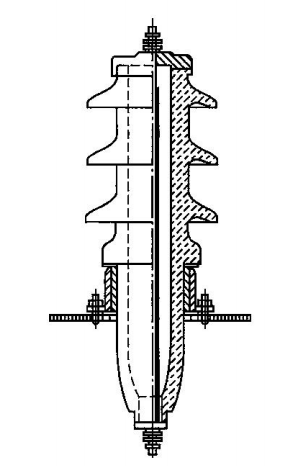
\includegraphics[width=2.2in]{2-9.png}  
		
		\caption{35kV瓷质充油式套管}
		\label{fig:2.9} 
	\end{minipage}
	\begin{minipage}[H]{0.4\linewidth}  
		\centering  
		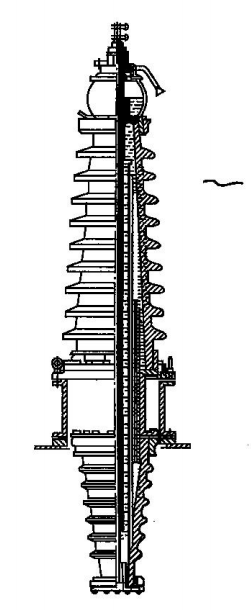
\includegraphics[width=2.2in]{2-10.png}  
		
		\caption{110kV电容式充油套管} 
		\label{fig:2.10} 
	\end{minipage}
\end{figure} 

\section{变压器的额定值}
为了保证变压器正常运行并有一定的使用寿命,在设计时对变压器的各主要物理量都要规定一个不许超过的限值,这就是它的额定值。变压器的额定值主要有以下几种。

(1)一次侧额定电压${{U}_{1N}}$和二次侧额定电压${{U}_{2N}}$:对于三相变压器${{U}_{1N}}$和${{U}_{2N}}$皆取线电压。

(2)一次侧额定电流${{I}_{1N}}$和二次侧额定电流${{I}_{2N}}$:对于三相变压器,${{I}_{1N}}$和${{I}_{2N}}$皆取线电流。

(3)额定电容${{S}_{N}}$:对于单相变压器有
\begin{equation}
{{S}_{N}}\text{=}{{U}_{1N}}{{I}_{1N}}={{U}_{2N}}{{I}_{2N}}
\label{1-1}
\end{equation}
对于三相变压器,有
\begin{equation}
{{S}_{N}}\text{=}\sqrt{3}{{U}_{1N}}{{I}_{1N}}=\sqrt{3}{{U}_{2N}}{{I}_{2N}}
\label{1-2}
\end{equation}
变压器一、二次侧额定视在功率相等,但在实际运行中输出功率和输入功率不可能完全相等。当变压器输出额定视在功率时,输入的视在功率将大于额定值。由于电力变压器效率很高,输出和输入功率相差很小。

(4)额定功率${{f}_{N}}$:我国规定工频为50Hz。

除了上述额定值外,在变压器铭牌上还标注有相数、额定效率和额定温升等数据。变压 器的额定容量决定着其铁心尺寸的大小,额定电压决定着绕组的匝数,额定电流决定着绕组导线截面的大小。

\section{小结}
(1) 变压器的种类繁多,而本节重点研究的是应用普遍的双绕组电力变压器。

(2) 作为磁路,变压器的铁心应具有良好的导磁性能和与其额定容量相对应的横截面积。

(3) 作为电路,变压器的绕组应具有良好的导电性,其匝数取决于变压器的额定电压,导线的截面积取决于变压器的额定电流。

(4) 变压器油具有散热和绝缘两种作用。根据散热的需要,变压器油箱可有多种不同的结构方式。

(5) 为了保证电力变压器安全可靠地运行,在其油箱盖上安装有多种辅助部件。

(6) 为了正确地选择和使用变压器,必须了解它的额定值,应注意的是,三相变压器的${{U}_{1N}}$、${{I}_{1N}}$皆指线值。




\end{document}